\documentclass[10pt,handout]{beamer}\usepackage{graphicx, color}
%% maxwidth is the original width if it is less than linewidth
%% otherwise use linewidth (to make sure the graphics do not exceed the margin)
\makeatletter
\def\maxwidth{ %
  \ifdim\Gin@nat@width>\linewidth
    \linewidth
  \else
    \Gin@nat@width
  \fi
}
\makeatother

\definecolor{fgcolor}{rgb}{0.2, 0.2, 0.2}
\newcommand{\hlfunctioncall}[1]{\textcolor[rgb]{0,0,0.545098039215686}{\textbf{#1}}}%
\newcommand{\hlstring}[1]{\textcolor[rgb]{0.282352941176471,0.23921568627451,0.545098039215686}{#1}}%
\newcommand{\hlnumber}[1]{\textcolor[rgb]{0,0,0}{#1}}%
\newcommand{\hlkeyword}[1]{\textcolor[rgb]{0,0,0}{\textbf{#1}}}%
\newcommand{\hlargument}[1]{\textcolor[rgb]{0.690196078431373,0.250980392156863,0.0196078431372549}{#1}}%
\newcommand{\hlcomment}[1]{\textcolor[rgb]{0.2,0.2,0.2}{#1}}%
\newcommand{\hlroxygencomment}[1]{\textcolor[rgb]{0.2,0.2,0.2}{#1}}%
\newcommand{\hlformalargs}[1]{\textcolor[rgb]{0.690196078431373,0.250980392156863,0.0196078431372549}{#1}}%
\newcommand{\hleqformalargs}[1]{\textcolor[rgb]{0.690196078431373,0.250980392156863,0.0196078431372549}{#1}}%
\newcommand{\hlassignement}[1]{\textcolor[rgb]{0,0,0}{\textbf{#1}}}%
\newcommand{\hlpackage}[1]{\textcolor[rgb]{0.588235294117647,0.709803921568627,0.145098039215686}{#1}}%
\newcommand{\hlslot}[1]{\textit{#1}}%
\newcommand{\hlsymbol}[1]{\textcolor[rgb]{0,0,0}{#1}}%
\newcommand{\hlprompt}[1]{\textcolor[rgb]{0.2,0.2,0.2}{#1}}%

\usepackage{framed}
\makeatletter
\newenvironment{kframe}{%
 \def\at@end@of@kframe{}%
 \ifinner\ifhmode%
  \def\at@end@of@kframe{\end{minipage}}%
  \begin{minipage}{\columnwidth}%
 \fi\fi%
 \def\FrameCommand##1{\hskip\@totalleftmargin \hskip-\fboxsep
 \colorbox{shadecolor}{##1}\hskip-\fboxsep
     % There is no \\@totalrightmargin, so:
     \hskip-\linewidth \hskip-\@totalleftmargin \hskip\columnwidth}%
 \MakeFramed {\advance\hsize-\width
   \@totalleftmargin\z@ \linewidth\hsize
   \@setminipage}}%
 {\par\unskip\endMakeFramed%
 \at@end@of@kframe}
\makeatother

\definecolor{shadecolor}{rgb}{.97, .97, .97}
\definecolor{messagecolor}{rgb}{0, 0, 0}
\definecolor{warningcolor}{rgb}{1, 0, 1}
\definecolor{errorcolor}{rgb}{1, 0, 0}
\newenvironment{knitrout}{}{} % an empty environment to be redefined in TeX

\usepackage{alltt}

\usetheme[compress]{PaloAlto}
\usecolortheme{sidebartab}
%\logo{\includegraphics[width=1cm]{../Rlogo-5.png}}

\usepackage[brazilian]{babel}
\usepackage[T1]{fontenc}
\usepackage[utf8]{inputenc}
\usepackage{graphicx}
\usepackage{hyperref}
\usepackage[scaled]{beramono} % truetype: Bistream Vera Sans Mono
%\usepackage{inconsolata}

\setbeamertemplate{footline}[frame number] % mostra o numero dos slides
\setbeamertemplate{navigation symbols}{} % retira a barra de navegacao

\usepackage{xspace}
\providecommand{\eg}{\textit{e.g.}\xspace}
\providecommand{\ie}{\textit{i.e.}\xspace}
%\providecommand{\R}{\texttt{R}\xspace}


\title{Introdução ao uso do R}

\title[Módulo I\\ Básico]{Introdução ao uso do software R}
\author[]{Fernando de Pol Mayer\inst{1} \and %\url{fernandomayer@gmail.com} \and
Rodrigo Sant'Ana\inst{2}} %\\ \url{oc.rodrigosantana@gmail.com}}
\date{26 e 27 de Novembro, 2012}
\institute{
  \inst{1}%
  Universidade Federal de Santa Catarina (UFSC) \\
  Departamento de Ecologia e Zoologia (ECZ/CCB) \\
  \url{fernando.mayer@gmail.com}
  \and
  \inst{2}%
  Instituto Albatroz \\
  \url{oc.rodrigosantana@gmail.com}
}
\logo{\includegraphics[width=1cm]{../Rlogo-5}}

% \author[Módulo I]{Fernando de Pol
%   Mayer\\ \texttt{fernando.mayer@ufsc.br}}
% \institute[Universidade Federal de Santa Catarina (UFSC)]{Departamento
%   de Ecologia e Zoologia (ECZ) \\ Universidade Federal de Santa Catarina
%   (UFSC)}
 % \date{3 de Outubro, 2012}

\AtBeginSection[]
{
  \begin{frame}
    \frametitle{Sumário}
    \tableofcontents[currentsection]
  \end{frame}
}

\AtBeginSubsection[]
{
  \begin{frame}
    \frametitle{Sumário}
    \tableofcontents[currentsection,currentsubsection]
  \end{frame}
}

\begin{document}




\begin{frame}
\maketitle
%\titlepage
\end{frame}

\begin{frame}{Sumário}
\tableofcontents
\end{frame}

\section{Introdução}

\begin{frame}{Histórico}
\begin{itemize}
\item[1980] Linguagem S: desenvolvida por R. Becker, J. Chambers e
  A. Wilks (AT\&T Bell Laboratories)
\item[1980] Versão comercial: S-Plus (Insightful Corporation)
\item[1996] Versão livre: R desenvolvido por R. Ihaka e R. Gentleman
  (Universidade de Auckland)
\end{itemize}
\end{frame}

\begin{frame}{Histórico}
\begin{itemize}
\item[1997] R Development Core Team
\item[Hoje] 20 desenvolvedores principais e muitos outros colaboradores
  em todo o mundo
\item[-] Estatísticos, matemáticos e programadores
\end{itemize}
\end{frame}

\begin{frame}{O que é o R?}
\begin{itemize}
\item Programa estatístico para análise de dados e produção de
  gráficos\pause
\item Uma completa linguagem de programação:
    \begin{itemize}
    \item Interpretada (contrário de compilada)\pause
    \item Orientada a objetos:
    \end{itemize}
\begin{quote}
    ``Tudo no R é um objeto\ldots''
\end{quote}\pause
\item Livre distribuição (código-aberto)\pause
\item Mais de 2000 pacotes adicionais\pause
\item Disponível em \url{http://www.R-project.org} \pause
\item Versão atual: 2.15.2 (26/10/2012). Ciclo de lançamentos: 6 meses
  (versões menores), 1 ano (versões maiores).
\end{itemize}
\end{frame}

\begin{frame}{Vantagens}
\begin{itemize}
\item Software livre
\item Funciona em praticamente todos os sistemas operacionais: Unix
  (Linux, FreeBSD, \ldots), Macintosh e Windows
\item É o produto da cooperação entre estatísticos do mundo todo
\item Linguagem lógica e intuitiva
\item Flexibilidade nas análises estatísticas
\item Gráficos de alta qualidade
\end{itemize}
\end{frame}

\begin{frame}{Desvantagens}
\begin{itemize}
\item Sem interface gráfica (?)
\item Não há visualização direta dos dados
\item Curva de aprendizado longa
\item Pode ser lento com grandes (GB, TB, \ldots) bases de dados
  \begin{itemize}
  \item Necessidade de \textbf{vetorização}
  \end{itemize}
\end{itemize}
\end{frame}

\section{Configuração inicial}

\begin{frame}[fragile=singleslide]{Configurando o diretório de trabalho}
\begin{itemize}
\item O diretório de trabalho é uma pasta onde o R será
  direcionado. Todos os arquivos que serão importados (base de dados,
  \ldots) ou exportados (base de dados, gráficos, \ldots) por ele
  ficarão nesta pasta.
\item No sistema Windows, existem duas maneiras de configurar o
  diretório de trabalho (suponha que vamos usar a pasta
  \verb|C:\cursoR|):
\end{itemize}
\end{frame}

\begin{frame}[fragile=singleslide]{Configurando o diretório de trabalho}
\begin{enumerate}
\item Utilizando a função \texttt{setwd()} dentro do R:
\begin{verbatim}
> setwd("C:/cursoR")
\end{verbatim}
Note que a barra é invertida!
\item Pelo menu do RStudio em \texttt{Session > Set Working Directory >
  Choose Directory \ldots}
\end{enumerate}
Confira o diretório que está trabalhando com a função
\begin{knitrout}\small
\definecolor{shadecolor}{rgb}{0.933, 0.914, 0.914}\color{fgcolor}\begin{kframe}
\begin{alltt}
> \hlfunctioncall{getwd}()
\end{alltt}
\end{kframe}
\end{knitrout}

\end{frame}

\section{Visão geral}

% \begin{frame}{``Interface gráfica''}
% \begin{figure}[htp]
% \centering
% 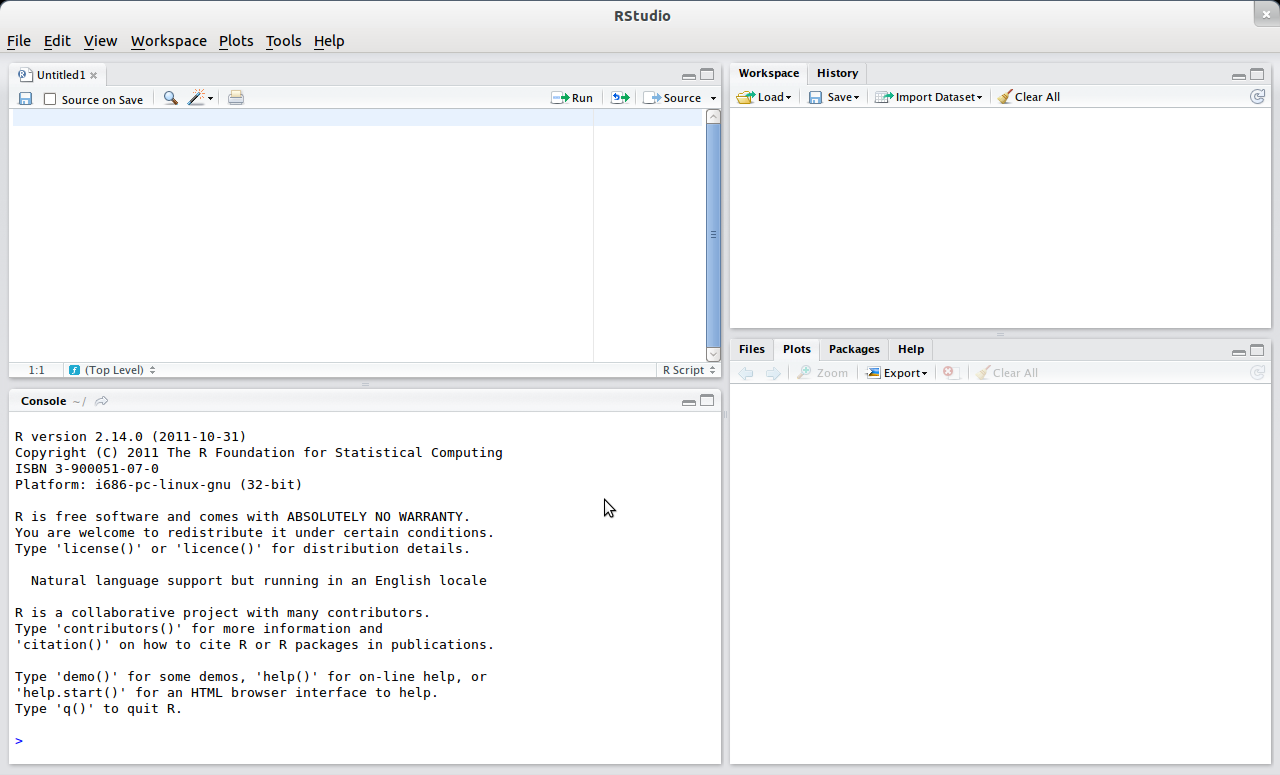
\includegraphics[width=0.9\textwidth]{RStudio_screen.png}
% \end{figure}
% \end{frame}

\begin{frame}[fragile=singleslide]{O R como uma calculadora}
O símbolo \verb|>| indica que o R está pronto para receber um comando:
\begin{knitrout}\small
\definecolor{shadecolor}{rgb}{0.933, 0.914, 0.914}\color{fgcolor}\begin{kframe}
\begin{alltt}
> 2 + 2
\end{alltt}
\begin{verbatim}
[1] 4
\end{verbatim}
\end{kframe}
\end{knitrout}

O símbolo \verb|>| muda para \verb|+| se o comando estiver incompleto:
\begin{knitrout}\small
\definecolor{shadecolor}{rgb}{0.933, 0.914, 0.914}\color{fgcolor}\begin{kframe}
\begin{alltt}
> 2 *
  2
\end{alltt}
\begin{verbatim}
[1] 4
\end{verbatim}
\end{kframe}
\end{knitrout}

Espaços entre os números não fazem diferença:
\begin{knitrout}\small
\definecolor{shadecolor}{rgb}{0.933, 0.914, 0.914}\color{fgcolor}\begin{kframe}
\begin{alltt}
> 2+         2
\end{alltt}
\begin{verbatim}
[1] 4
\end{verbatim}
\end{kframe}
\end{knitrout}

\end{frame}

\begin{frame}[fragile=singleslide]{O editor de scripts}
  \begin{itemize}
  \item Para criar rotinas computacionais é necessário utilizar um editor
    de scripts.
  \item Clique em \texttt{Arquivo > Novo script}. Salve com a extensão
    \texttt{.R}.
  \item Para enviar comandos diretamente para o console, selecione-os e
    aperte \texttt{Ctrl + R}.
  \item Para adicionar comentários ao script, utiliza-se o símbolo
    \texttt{\#} antes do texto e/ou comandos. O que estiver depois do
    símbolo não será interpretado pelo R. Portanto:
\begin{knitrout}\small
\definecolor{shadecolor}{rgb}{0.933, 0.914, 0.914}\color{fgcolor}\begin{kframe}
\begin{alltt}
2 + 2     \hlcomment{# esta linha será executada}
\hlcomment{# 2 + 2     esta linha não será executada}
\end{alltt}
\end{kframe}
\end{knitrout}

\end{itemize}
\end{frame}


\begin{frame}[fragile=singleslide]{Operadores aritméticos}
\begin{table}[!ht]
    \centering
    %\caption
        \begin{tabular}{cl}
        \hline
        \multicolumn{0}{c}{Operador} & \multicolumn{1}{c}{Significado} \\
        \hline
        \verb|+| & adição \\
        \verb|-| & subtração \\
        \verb|*| & multiplicação \\
        \verb|/| & divisão \\
        \verb|^| & potência \\
        \verb|exp()| & exponencial \\
        \verb|sqrt()| & raíz quadrada \\
        \verb|factorial()| & fatorial \\
        \verb|log(); log2(); log10()| & logaritmos \\
        \hline
        \end{tabular}
    %\label{tab:oper}
\end{table}
\end{frame}

\begin{frame}[fragile=singleslide]{Ordems de execução}
As operações são realizadas sempre seguindo as prioridades:
\begin{enumerate}
\item De dentro para fora de parênteses \verb|()|
\item Multiplicação e divisão
\item Adição e subtração
\end{enumerate}
\begin{knitrout}\small
\definecolor{shadecolor}{rgb}{0.933, 0.914, 0.914}\color{fgcolor}\begin{kframe}
\begin{alltt}
> 5 * 2 - 10 + 7
\end{alltt}
\begin{verbatim}
[1] 7
\end{verbatim}
\begin{alltt}
> 5 * 2 - (10 + 7)
\end{alltt}
\begin{verbatim}
[1] -7
\end{verbatim}
\begin{alltt}
> 5 * (2 - 10 + 7)
\end{alltt}
\begin{verbatim}
[1] -5
\end{verbatim}
\begin{alltt}
> 5 * (2 - (10 + 7))
\end{alltt}
\begin{verbatim}
[1] -75
\end{verbatim}
\end{kframe}
\end{knitrout}

\end{frame}

\section{Funções e argumentos}

\begin{frame}[fragile=singleslide]{Funções e argumentos}
As funções no R são definidas como:
\begin{knitrout}\small
\definecolor{shadecolor}{rgb}{0.933, 0.914, 0.914}\color{fgcolor}\begin{kframe}
\begin{alltt}
> \hlfunctioncall{nome}(argumento1, argumento2, ...)
\end{alltt}
\end{kframe}
\end{knitrout}

Exemplo: função \verb|runif()| (para gerar valores aleatórios de uma
distribuição uniforme):
\begin{knitrout}\small
\definecolor{shadecolor}{rgb}{0.933, 0.914, 0.914}\color{fgcolor}\begin{kframe}
\begin{alltt}
> \hlfunctioncall{runif}(n, min = 0, max = 1)
\end{alltt}
\end{kframe}
\end{knitrout}

\begin{knitrout}\small
\definecolor{shadecolor}{rgb}{0.933, 0.914, 0.914}\color{fgcolor}\begin{kframe}
\begin{alltt}
> \hlfunctioncall{runif}(10, 1, 100)
\end{alltt}
\begin{verbatim}
 [1] 78.2667 84.0486 76.2982 11.8207 27.1370  2.7101 30.6247
 [8] 18.6032 60.2046 71.1004
\end{verbatim}
\end{kframe}
\end{knitrout}

\end{frame}

\begin{frame}[fragile=singleslide]{Funções e argumentos}
Argumentos que já possuem um valor especificado (como \texttt{max} e
\texttt{min}) podem ser omitidos:
\begin{knitrout}\small
\definecolor{shadecolor}{rgb}{0.933, 0.914, 0.914}\color{fgcolor}\begin{kframe}
\begin{alltt}
> \hlfunctioncall{runif}(10)
\end{alltt}
\end{kframe}
\end{knitrout}

Se os argumentos forem nomeados, a ordem deles dentro da função não tem
mais importância:
\begin{knitrout}\small
\definecolor{shadecolor}{rgb}{0.933, 0.914, 0.914}\color{fgcolor}\begin{kframe}
\begin{alltt}
> \hlfunctioncall{runif}(min = 1, max = 100, n = 10)
\end{alltt}
\end{kframe}
\end{knitrout}

Argumentos nomeados e não nomeados podem ser utilizados, desde que os
não nomeados estejam na posição correta:
\begin{knitrout}\small
\definecolor{shadecolor}{rgb}{0.933, 0.914, 0.914}\color{fgcolor}\begin{kframe}
\begin{alltt}
> \hlfunctioncall{runif}(10, max = 100, min = 1)
\end{alltt}
\end{kframe}
\end{knitrout}

\end{frame}

\begin{frame}[fragile=singleslide]{Outros tipos de argumentos}
Exemplo: função \verb|sample()|:
\begin{knitrout}\small
\definecolor{shadecolor}{rgb}{0.933, 0.914, 0.914}\color{fgcolor}\begin{kframe}
\begin{alltt}
> \hlfunctioncall{sample}(x, size, replace = FALSE, prob = NULL)
\end{alltt}
\end{kframe}
\end{knitrout}

\begin{itemize}
\item \verb|x| e \verb|size| devem ser obrigatoriamente especificados
\item \verb|replace| é lógico: \verb|TRUE| (\verb|T|) ou \verb|FALSE|
  (\verb|F|)
\item \verb|prob| é um argumento vazio ou ausente (``opcional'')
\end{itemize}
Exemplo: função \verb|plot()|:
\begin{knitrout}\small
\definecolor{shadecolor}{rgb}{0.933, 0.914, 0.914}\color{fgcolor}\begin{kframe}
\begin{alltt}
> \hlfunctioncall{plot}(x, y, ...)
\end{alltt}
\end{kframe}
\end{knitrout}

\begin{itemize}
\item ``\ldots'' permite especificar argumentos de outras funções (por
  exemplo \verb|par()|)
\end{itemize}
\end{frame}

\begin{frame}[fragile=singleslide]{Exercícios}
  \begin{enumerate}
  \item Calcule a seguinte equação: $32 + 16^2 - 25^3$
  \item Divida o resultado por $345$
  \item Qual o resultado da expressão $\frac{e^{-2}  2^{4} - 1}{4!}$?
  \item E do logaritmo desta expressão?
  \item Usando a função \verb|runif()| gere $30$ números aleatórios entre:
    \begin{itemize}
    \item 0 e 1
    \item -5 e 5
    \item 10 e 500
    \end{itemize}
  \end{enumerate}
\end{frame}

\begin{frame}[fragile=singleslide]{Mecanismos de ajuda}
Argumentos e detalhes do funcionamento das funções:
\begin{knitrout}\small
\definecolor{shadecolor}{rgb}{0.933, 0.914, 0.914}\color{fgcolor}\begin{kframe}
\begin{alltt}
> ?runif
\end{alltt}
\end{kframe}
\end{knitrout}

ou
\begin{knitrout}\small
\definecolor{shadecolor}{rgb}{0.933, 0.914, 0.914}\color{fgcolor}\begin{kframe}
\begin{alltt}
> \hlfunctioncall{help}(runif)
\end{alltt}
\end{kframe}
\end{knitrout}

A documentação contém os campos:
\begin{itemize}
\item \textbf{Description:} breve descrição
\item \textbf{Usage:} função e todos seus argumentos
\item \textbf{Arguments:} lista descrevendo cada argumento
\item \textbf{Details:} descrição detalhada
\item \textbf{Value:} o que a função retorna
\item \textbf{References:} bibliografia relacionada
\item \textbf{See Also:} funções relacionadas
\item \textbf{Examples:} exemplos práticos
\end{itemize}
\end{frame}

\begin{frame}[fragile=singleslide]{Mecanismos de ajuda}
Procura por funções que contenham \texttt{"palavra"}:
\begin{knitrout}\small
\definecolor{shadecolor}{rgb}{0.933, 0.914, 0.914}\color{fgcolor}\begin{kframe}
\begin{alltt}
> \hlfunctioncall{help.search}(\hlstring{"palavra"})
\end{alltt}
\end{kframe}
\end{knitrout}

Ajuda através do navegador (também contém manuais, \ldots):
\begin{knitrout}\small
\definecolor{shadecolor}{rgb}{0.933, 0.914, 0.914}\color{fgcolor}\begin{kframe}
\begin{alltt}
> \hlfunctioncall{help.start}()
\end{alltt}
\end{kframe}
\end{knitrout}

Busca por \texttt{"palavra"} nos arquivos da lista de discussão do R:
\begin{knitrout}\small
\definecolor{shadecolor}{rgb}{0.933, 0.914, 0.914}\color{fgcolor}\begin{kframe}
\begin{alltt}
> \hlfunctioncall{RSiteSearch}(\hlstring{"palavra"})
\end{alltt}
\end{kframe}
\end{knitrout}

\end{frame}

\section{Objetos}

\begin{frame}[fragile=singleslide]{Programação orientada a objetos}
O que é um objeto?
\begin{itemize}
\item Um \textbf{símbolo} ou uma \textbf{variável} capaz de armazenar
  qualquer valor ou estrutura de dados
\end{itemize}
Por quê objetos?
\begin{itemize}
\item Uma maneira simples de acessar os dados armazenados na memória (o
  R não permite acesso direto à memória)
\end{itemize}
Programação:
\begin{itemize}
\item Objetos $\rightarrow$ Classes $\rightarrow$ Métodos
\end{itemize}
\end{frame}

\begin{frame}[fragile=singleslide]{Objetos}
\begin{quote}
    ``Tudo no R é um objeto.''\\
    ``Todo objeto no R tem uma classe''
\end{quote}
\begin{itemize}
\item \textbf{Classe:} é a definição de um objeto. Descreve a forma do
  objeto e como ele será manipulado pelas diferentes funções
\item \textbf{Método:} são \textbf{funções genéricas} que executam suas
  tarefas de acordo com cada classe. As funções genéricas mais
  importantes são:
  \begin{itemize}
  \item \verb|summary()|
  \item \verb|plot()|
  \end{itemize}
\end{itemize}
\end{frame}

\begin{frame}[fragile=singleslide]{Objetos}
A variável \texttt{x} recebe o valor $2$ (tornando-se um objeto dentro do R):
\begin{knitrout}\small
\definecolor{shadecolor}{rgb}{0.933, 0.914, 0.914}\color{fgcolor}\begin{kframe}
\begin{alltt}
> x <- 2
\end{alltt}
\end{kframe}
\end{knitrout}

\begin{center}
\fbox{\parbox{0.9\textwidth}{O símbolo \texttt{<-} é chamado de
    \textbf{operador de atribuição}. Ele serve para atribuir valores a
    objetos, e é formado pelos símbolos \texttt{<} e \texttt{-},
    obrigatoriamente \emph{sem espaços}.}}
\end{center}
Para ver o conteúdo do objeto:
\begin{knitrout}\small
\definecolor{shadecolor}{rgb}{0.933, 0.914, 0.914}\color{fgcolor}\begin{kframe}
\begin{alltt}
> x
\end{alltt}
\begin{verbatim}
[1] 2
\end{verbatim}
\end{kframe}
\end{knitrout}

Obs.: O símbolo \verb|=| pode ser usado no lugar de \verb|<-| mas não é
recomendado.
\end{frame}

\begin{frame}[fragile=singleslide]{Objetos}
Quando você faz
\begin{knitrout}\small
\definecolor{shadecolor}{rgb}{0.933, 0.914, 0.914}\color{fgcolor}\begin{kframe}
\begin{alltt}
> x <- 2
\end{alltt}
\end{kframe}
\end{knitrout}

está fazendo uma \textbf{declaração}, ou seja, declarando que a variável
\verb|x| irá agora se tornar um objeto que armazena o número
\verb|2|. As declarações podem ser feitas uma em cada linha
\begin{knitrout}\small
\definecolor{shadecolor}{rgb}{0.933, 0.914, 0.914}\color{fgcolor}\begin{kframe}
\begin{alltt}
> x <- 2
> y <- 4
\end{alltt}
\end{kframe}
\end{knitrout}

ou separadas por \verb|;|
\begin{knitrout}\small
\definecolor{shadecolor}{rgb}{0.933, 0.914, 0.914}\color{fgcolor}\begin{kframe}
\begin{alltt}
> x <- 2; y <- 4
\end{alltt}
\end{kframe}
\end{knitrout}

\end{frame}

\begin{frame}[fragile=singleslide]{Objetos}
Operações matemáticas em objetos:
\begin{knitrout}\small
\definecolor{shadecolor}{rgb}{0.933, 0.914, 0.914}\color{fgcolor}\begin{kframe}
\begin{alltt}
> x + x
\end{alltt}
\begin{verbatim}
[1] 4
\end{verbatim}
\end{kframe}
\end{knitrout}

Objetos podem armazenar diferentes estruturas de dados:
\begin{knitrout}\small
\definecolor{shadecolor}{rgb}{0.933, 0.914, 0.914}\color{fgcolor}\begin{kframe}
\begin{alltt}
> y <- \hlfunctioncall{runif}(10)
> y
\end{alltt}
\begin{verbatim}
 [1] 0.374754 0.065701 0.681238 0.152589 0.059587 0.446746
 [7] 0.251067 0.929592 0.437038 0.665539
\end{verbatim}
\end{kframe}
\end{knitrout}

Note que cada objeto só pode armazenar uma estrutura (um número ou uma
sequência de valores) de cada vez! (Aqui, o valor $4$ que estava
armazenado em \verb|y| foi sobrescrito pelos valores acima.)
\end{frame}

\begin{frame}[fragile=singleslide]{Nomes de objetos}
\begin{itemize}
\item Podem ser formados por letras, números e ``\texttt{.}'' (ponto)
\item Não podem começar com número e/ou ponto
\item Não podem conter espaços
\item Evite usar acentos
\item Evite usar nomes de funções como:
\end{itemize}
\begin{quote}
\begin{center}
\ttfamily \upshape
c q t C D F I T diff df data var pt
\end{center}
\end{quote}
\begin{itemize}
\item O R é \emph{case-sensitive}, portanto:
\end{itemize}
\begin{quote}
\begin{center}
\ttfamily \upshape
\texttt{dados} $\neq$ \texttt{Dados} $\neq$ \texttt{DADOS}
\end{center}
\end{quote}
\end{frame}

\begin{frame}[fragile=singleslide]{Gerenciando a área de trabalho (\textit{workspace})}
Liste os objetos criados com a função \texttt{ls()}:
\begin{knitrout}\small
\definecolor{shadecolor}{rgb}{0.933, 0.914, 0.914}\color{fgcolor}\begin{kframe}
\begin{alltt}
> \hlfunctioncall{ls}()
\end{alltt}
\end{kframe}
\end{knitrout}

Para remover apenas um objeto:
\begin{knitrout}\small
\definecolor{shadecolor}{rgb}{0.933, 0.914, 0.914}\color{fgcolor}\begin{kframe}
\begin{alltt}
> \hlfunctioncall{rm}(x)
\end{alltt}
\end{kframe}
\end{knitrout}

Para remover outros objetos:
\begin{knitrout}\small
\definecolor{shadecolor}{rgb}{0.933, 0.914, 0.914}\color{fgcolor}\begin{kframe}
\begin{alltt}
> \hlfunctioncall{rm}(x, y)
\end{alltt}
\end{kframe}
\end{knitrout}

Para remover todos os objetos:
\begin{knitrout}\small
\definecolor{shadecolor}{rgb}{0.933, 0.914, 0.914}\color{fgcolor}\begin{kframe}
\begin{alltt}
> \hlfunctioncall{rm}(list = \hlfunctioncall{ls}())
\end{alltt}
\end{kframe}
\end{knitrout}

\end{frame}

\begin{frame}[fragile=singleslide]{Exercícios}
  \begin{enumerate}
  \item Armazene o resultado da equação $32 + 16^2 - 25^3$ no objeto
    \verb|x|
  \item Divida \verb|x| por $345$ e armazene em \verb|y|
  \item Crie um objeto (com o nome que você quiser) para armazenar $30$
    valores aleatórios de uma distribuição uniforme entre $10$ e $50$
  \item Remova o objeto \verb|y|
  \item Remova os demais objetos de uma única vez
  \end{enumerate}
\end{frame}

\subsection[Classes]{Classes de objetos}

\begin{frame}[fragile=singleslide]{Vetor}
Características:
\begin{itemize}
\item Coleção ordenada de valores
\item Estrutura unidimensional
\end{itemize}
Usando a função \texttt{c()} para criar vetores:
\begin{knitrout}\small
\definecolor{shadecolor}{rgb}{0.933, 0.914, 0.914}\color{fgcolor}\begin{kframe}
\begin{alltt}
> numerico <- \hlfunctioncall{c}(10, 5, 2, 4, 8, 9)
> numerico
\end{alltt}
\begin{verbatim}
[1] 10  5  2  4  8  9
\end{verbatim}
\end{kframe}
\end{knitrout}

\end{frame}

\begin{frame}[fragile=singleslide]{Vetor}{Sequências de números}
  Usando a função \verb|seq()|
\begin{knitrout}\small
\definecolor{shadecolor}{rgb}{0.933, 0.914, 0.914}\color{fgcolor}\begin{kframe}
\begin{alltt}
> \hlfunctioncall{seq}(1, 10)
\end{alltt}
\begin{verbatim}
 [1]  1  2  3  4  5  6  7  8  9 10
\end{verbatim}
\end{kframe}
\end{knitrout}

Ou \verb|1:10| gera o mesmo resultado. Para a sequência variar em $2$
\begin{knitrout}\small
\definecolor{shadecolor}{rgb}{0.933, 0.914, 0.914}\color{fgcolor}\begin{kframe}
\begin{alltt}
> \hlfunctioncall{seq}(from = 1, to = 10, by = 2)
\end{alltt}
\begin{verbatim}
[1] 1 3 5 7 9
\end{verbatim}
\end{kframe}
\end{knitrout}

Para obter $15$ valores entre $1$ e $10$
\begin{knitrout}\small
\definecolor{shadecolor}{rgb}{0.933, 0.914, 0.914}\color{fgcolor}\begin{kframe}
\begin{alltt}
> \hlfunctioncall{seq}(from = 1, to = 10, length.out = 15)
\end{alltt}
\begin{verbatim}
 [1]  1.0000  1.6429  2.2857  2.9286  3.5714  4.2143  4.8571
 [8]  5.5000  6.1429  6.7857  7.4286  8.0714  8.7143  9.3571
[15] 10.0000
\end{verbatim}
\end{kframe}
\end{knitrout}

\end{frame}

\begin{frame}[fragile=singleslide]{Vetor}{Sequências de números}
  Usando a função \verb|rep()|
\begin{knitrout}\small
\definecolor{shadecolor}{rgb}{0.933, 0.914, 0.914}\color{fgcolor}\begin{kframe}
\begin{alltt}
> \hlfunctioncall{rep}(1, 10)
\end{alltt}
\begin{verbatim}
 [1] 1 1 1 1 1 1 1 1 1 1
\end{verbatim}
\end{kframe}
\end{knitrout}

Para gerar um sequência várias vezes
\begin{knitrout}\small
\definecolor{shadecolor}{rgb}{0.933, 0.914, 0.914}\color{fgcolor}\begin{kframe}
\begin{alltt}
> \hlfunctioncall{rep}(\hlfunctioncall{c}(1, 2, 3), 5)
\end{alltt}
\begin{verbatim}
 [1] 1 2 3 1 2 3 1 2 3 1 2 3 1 2 3
\end{verbatim}
\end{kframe}
\end{knitrout}

Para repetir um número da sequência várias vezes
\begin{knitrout}\small
\definecolor{shadecolor}{rgb}{0.933, 0.914, 0.914}\color{fgcolor}\begin{kframe}
\begin{alltt}
> \hlfunctioncall{rep}(\hlfunctioncall{c}(1, 2, 3), each = 5)
\end{alltt}
\begin{verbatim}
 [1] 1 1 1 1 1 2 2 2 2 2 3 3 3 3 3
\end{verbatim}
\end{kframe}
\end{knitrout}

\end{frame}

\begin{frame}[fragile=singleslide]{Vetor}{Operações matemáticas em vetores}
Operações podem ser feitas entre um vetor e um número:
\begin{knitrout}\small
\definecolor{shadecolor}{rgb}{0.933, 0.914, 0.914}\color{fgcolor}\begin{kframe}
\begin{alltt}
> numerico * 2
\end{alltt}
\begin{verbatim}
[1] 20 10  4  8 16 18
\end{verbatim}
\end{kframe}
\end{knitrout}

E também entre vetores de mesmo comprimento ou com comprimentos
múltiplos:
\begin{knitrout}\small
\definecolor{shadecolor}{rgb}{0.933, 0.914, 0.914}\color{fgcolor}\begin{kframe}
\begin{alltt}
> numerico * numerico
\end{alltt}
\begin{verbatim}
[1] 100  25   4  16  64  81
\end{verbatim}
\begin{alltt}
> numerico + \hlfunctioncall{c}(2, 4, 1)
\end{alltt}
\begin{verbatim}
[1] 12  9  3  6 12 10
\end{verbatim}
\end{kframe}
\end{knitrout}

\end{frame}

\begin{frame}[fragile=singleslide]{Vetor}
A Regra da Reciclagem
\begin{table}[htbp]
%\caption{}
\begin{center}
\begin{tabular}{|c|c|c|c|c|c|}
\hline
\multicolumn{ 2}{|c|}{Original} & \multicolumn{ 2}{c|}{Expandido} & \multicolumn{ 2}{c|}{Resposta} \\ \hline
numerico & c(2,4,1) & numerico & c(2,4,1) & \multicolumn{ 2}{c|}{numerico + c(2,4,1)} \\ \hline
10 & 2 & 10 & 2 & \multicolumn{ 2}{c|}{12} \\ \hline
5 & 4 & 5 & 4 & \multicolumn{ 2}{c|}{9} \\ \hline
2 & 1 & 2 & 1 & \multicolumn{ 2}{c|}{3} \\ \hline
4 &  & 4 & 2 & \multicolumn{ 2}{c|}{6} \\ \hline
8 &  & 8 & 4 & \multicolumn{ 2}{c|}{12} \\ \hline
9 &  & 9 & 1 & \multicolumn{ 2}{c|}{10} \\ \hline
\end{tabular}
\end{center}
%\label{}
\end{table}
Agora tente:
\begin{knitrout}\small
\definecolor{shadecolor}{rgb}{0.933, 0.914, 0.914}\color{fgcolor}\begin{kframe}
\begin{alltt}
> numerico + \hlfunctioncall{c}(2, 4, 1, 3)
\end{alltt}
\end{kframe}
\end{knitrout}


\end{frame}

\begin{frame}[fragile=singleslide]{Vetor}{Atributos de objetos}
Classe:
\begin{knitrout}\small
\definecolor{shadecolor}{rgb}{0.933, 0.914, 0.914}\color{fgcolor}\begin{kframe}
\begin{alltt}
> \hlfunctioncall{class}(numerico)
\end{alltt}
\begin{verbatim}
[1] "numeric"
\end{verbatim}
\end{kframe}
\end{knitrout}

Comprimento:
\begin{knitrout}\small
\definecolor{shadecolor}{rgb}{0.933, 0.914, 0.914}\color{fgcolor}\begin{kframe}
\begin{alltt}
> \hlfunctioncall{length}(numerico)
\end{alltt}
\begin{verbatim}
[1] 6
\end{verbatim}
\end{kframe}
\end{knitrout}

\end{frame}

\begin{frame}[fragile=singleslide]{Vetor}
Vetores também podem ter outras classes:
\begin{itemize}
\item Vetor de caracteres:
\begin{knitrout}\small
\definecolor{shadecolor}{rgb}{0.933, 0.914, 0.914}\color{fgcolor}\begin{kframe}
\begin{alltt}
> caracter <- \hlfunctioncall{c}(\hlstring{"brava"}, \hlstring{"joaquina"}, \hlstring{"armação"})
> caracter
\end{alltt}
\begin{verbatim}
[1] "brava"    "joaquina" "armação" 
\end{verbatim}
\end{kframe}
\end{knitrout}

\item Vetor lógico:
\begin{knitrout}\small
\definecolor{shadecolor}{rgb}{0.933, 0.914, 0.914}\color{fgcolor}\begin{kframe}
\begin{alltt}
> logico <- caracter == \hlstring{"armação"}
> logico
\end{alltt}
\begin{verbatim}
[1] FALSE FALSE  TRUE
\end{verbatim}
\end{kframe}
\end{knitrout}

ou
\begin{knitrout}\small
\definecolor{shadecolor}{rgb}{0.933, 0.914, 0.914}\color{fgcolor}\begin{kframe}
\begin{alltt}
> logico <- numerico > 4
> logico
\end{alltt}
\begin{verbatim}
[1]  TRUE  TRUE FALSE FALSE  TRUE  TRUE
\end{verbatim}
\end{kframe}
\end{knitrout}

\end{itemize}
\end{frame}

\begin{frame}[fragile=singleslide]{Vetor}
No exemplo anterior, a condição \texttt{numerico > 4} é uma
\textbf{expressão condicional}, e o símbolo \texttt{>} um
\textbf{operador lógico}. Os operadores lógicos utilizados no R são:

\begin{table}[!ht]
    \centering
    %\caption
        \begin{tabular}{cl}
        \hline
        \multicolumn{0}{c}{Operador} & \multicolumn{1}{c}{Significado} \\
        \hline
        \verb|<| & menor \\
        \verb|<=| & menor igual \\
        \verb|>| & maior \\
        \verb|>=| & maior igual \\
        \verb|==| & igual \\
        \verb|!=| & diferente \\
        \verb|&| & e \\
        \verb+|+ & ou \\
        \hline
        \end{tabular}
    %\label{tab:oper}
\end{table}
\end{frame}

\begin{frame}[fragile=singleslide]{Fator}
Características:
\begin{itemize}
\item Coleção de categorias ou \textbf{níveis} (\emph{levels})
\item Estrutura unidimensional
\end{itemize}
Utilizando as funções \texttt{factor()} e \texttt{c()}:
\begin{knitrout}\small
\definecolor{shadecolor}{rgb}{0.933, 0.914, 0.914}\color{fgcolor}\begin{kframe}
\begin{alltt}
> fator <- \hlfunctioncall{factor}(\hlfunctioncall{c}(\hlstring{"alta"},\hlstring{"baixa"},\hlstring{"baixa"},\hlstring{"media"},
                    \hlstring{"alta"},\hlstring{"media"},\hlstring{"baixa"},\hlstring{"media"},\hlstring{"media"}))
> fator
\end{alltt}
\begin{verbatim}
[1] alta  baixa baixa media alta  media baixa media media
Levels: alta baixa media
\end{verbatim}
\begin{alltt}
> \hlfunctioncall{class}(fator)
\end{alltt}
\begin{verbatim}
[1] "factor"
\end{verbatim}
\end{kframe}
\end{knitrout}

\end{frame}

\begin{frame}[fragile=singleslide]{Fator}
Caso haja uma hierarquia, os níveis dos fatores podem ser ordenados:
\begin{knitrout}\small
\definecolor{shadecolor}{rgb}{0.933, 0.914, 0.914}\color{fgcolor}\begin{kframe}
\begin{alltt}
> fator <- \hlfunctioncall{factor}(\hlfunctioncall{c}(\hlstring{"alta"},\hlstring{"baixa"},\hlstring{"baixa"},\hlstring{"media"},
                    \hlstring{"alta"},\hlstring{"media"},\hlstring{"baixa"},\hlstring{"media"},\hlstring{"media"}),
                  levels=\hlfunctioncall{c}(\hlstring{"alta"},\hlstring{"media"},\hlstring{"baixa"}))
> fator
\end{alltt}
\begin{verbatim}
[1] alta  baixa baixa media alta  media baixa media media
Levels: alta media baixa
\end{verbatim}
\end{kframe}
\end{knitrout}

\end{frame}

\begin{frame}[fragile=singleslide]{Fator}{Transformando outras classes
    em fator e \textit{vice-versa}}
Numérico para fator:
\begin{knitrout}\small
\definecolor{shadecolor}{rgb}{0.933, 0.914, 0.914}\color{fgcolor}\begin{kframe}
\begin{alltt}
> num.fac <- \hlfunctioncall{as.factor}(numerico)
> num.fac
\end{alltt}
\begin{verbatim}
[1] 10 5  2  4  8  9 
Levels: 2 4 5 8 9 10
\end{verbatim}
\end{kframe}
\end{knitrout}

Fator para numérico:
\begin{knitrout}\small
\definecolor{shadecolor}{rgb}{0.933, 0.914, 0.914}\color{fgcolor}\begin{kframe}
\begin{alltt}
> num.num <- \hlfunctioncall{as.numeric}(\hlfunctioncall{as.character}(num.fac))
> num.num
\end{alltt}
\begin{verbatim}
[1] 10  5  2  4  8  9
\end{verbatim}
\end{kframe}
\end{knitrout}

Caracter para fator:
\begin{knitrout}\small
\definecolor{shadecolor}{rgb}{0.933, 0.914, 0.914}\color{fgcolor}\begin{kframe}
\begin{alltt}
> carac.fac <- \hlfunctioncall{as.factor}(caracter)
> carac.fac
\end{alltt}
\begin{verbatim}
[1] brava    joaquina armação 
Levels: armação brava joaquina
\end{verbatim}
\end{kframe}
\end{knitrout}

\end{frame}

\begin{frame}[fragile=singleslide]{Matriz}
Características:
\begin{itemize}
\item Podem conter apenas um tipo de informação (números, caracteres)
\item Estrutura bidimensional
\end{itemize}
Utilizando a função \texttt{matrix()}:
\begin{knitrout}\small
\definecolor{shadecolor}{rgb}{0.933, 0.914, 0.914}\color{fgcolor}\begin{kframe}
\begin{alltt}
> matriz <- \hlfunctioncall{matrix}(1:12, nrow=3, ncol=4)
> matriz
\end{alltt}
\begin{verbatim}
     [,1] [,2] [,3] [,4]
[1,]    1    4    7   10
[2,]    2    5    8   11
[3,]    3    6    9   12
\end{verbatim}
\begin{alltt}
> \hlfunctioncall{class}(matriz)
\end{alltt}
\begin{verbatim}
[1] "matrix"
\end{verbatim}
\end{kframe}
\end{knitrout}

\end{frame}

\begin{frame}[fragile=singleslide]{Matriz}
Alterando a ordem de preenchimento da matriz (por linhas):
\begin{knitrout}\small
\definecolor{shadecolor}{rgb}{0.933, 0.914, 0.914}\color{fgcolor}\begin{kframe}
\begin{alltt}
> matriz <- \hlfunctioncall{matrix}(1:12, nrow=3, ncol=4, byrow=T)
> matriz
\end{alltt}
\begin{verbatim}
     [,1] [,2] [,3] [,4]
[1,]    1    2    3    4
[2,]    5    6    7    8
[3,]    9   10   11   12
\end{verbatim}
\end{kframe}
\end{knitrout}

Para verificar a dimensão da matriz:
\begin{knitrout}\small
\definecolor{shadecolor}{rgb}{0.933, 0.914, 0.914}\color{fgcolor}\begin{kframe}
\begin{alltt}
> \hlfunctioncall{dim}(matriz)
\end{alltt}
\begin{verbatim}
[1] 3 4
\end{verbatim}
\end{kframe}
\end{knitrout}

\end{frame}

\begin{frame}[fragile=singleslide]{Matriz}
Adicionando colunas com \verb|cbind()|
\begin{knitrout}\small
\definecolor{shadecolor}{rgb}{0.933, 0.914, 0.914}\color{fgcolor}\begin{kframe}
\begin{alltt}
> \hlfunctioncall{cbind}(matriz, \hlfunctioncall{rep}(99, 3))
\end{alltt}
\begin{verbatim}
     [,1] [,2] [,3] [,4] [,5]
[1,]    1    2    3    4   99
[2,]    5    6    7    8   99
[3,]    9   10   11   12   99
\end{verbatim}
\end{kframe}
\end{knitrout}

Adicionando linhas com \verb|rbind()|
\begin{knitrout}\small
\definecolor{shadecolor}{rgb}{0.933, 0.914, 0.914}\color{fgcolor}\begin{kframe}
\begin{alltt}
> \hlfunctioncall{rbind}(matriz, \hlfunctioncall{rep}(99, 4))
\end{alltt}
\begin{verbatim}
     [,1] [,2] [,3] [,4]
[1,]    1    2    3    4
[2,]    5    6    7    8
[3,]    9   10   11   12
[4,]   99   99   99   99
\end{verbatim}
\end{kframe}
\end{knitrout}

\end{frame}

\begin{frame}[fragile=singleslide]{Matriz}{Operações matemáticas em
    matrizes}
Matriz multiplicada por um escalar
\begin{knitrout}\small
\definecolor{shadecolor}{rgb}{0.933, 0.914, 0.914}\color{fgcolor}\begin{kframe}
\begin{alltt}
> matriz * 2
\end{alltt}
\begin{verbatim}
     [,1] [,2] [,3] [,4]
[1,]    2    4    6    8
[2,]   10   12   14   16
[3,]   18   20   22   24
\end{verbatim}
\end{kframe}
\end{knitrout}

Multiplicação de matrizes (observe as dimensões!)
\begin{knitrout}\small
\definecolor{shadecolor}{rgb}{0.933, 0.914, 0.914}\color{fgcolor}\begin{kframe}
\begin{alltt}
> matriz2 <- \hlfunctioncall{matrix}(1, nrow=4, ncol=3)
> matriz %*% matriz2
\end{alltt}
\begin{verbatim}
     [,1] [,2] [,3]
[1,]   10   10   10
[2,]   26   26   26
[3,]   42   42   42
\end{verbatim}
\end{kframe}
\end{knitrout}

\end{frame}

\begin{frame}[fragile=singleslide]{Matriz}
Associando nomes às linhas e colunas:
\begin{knitrout}\small
\definecolor{shadecolor}{rgb}{0.933, 0.914, 0.914}\color{fgcolor}\begin{kframe}
\begin{alltt}
> \hlfunctioncall{rownames}(matriz) <- \hlfunctioncall{c}(\hlstring{"A"},\hlstring{"B"},\hlstring{"C"})
> \hlfunctioncall{colnames}(matriz) <- \hlfunctioncall{c}(\hlstring{"T1"},\hlstring{"T2"},\hlstring{"T3"},\hlstring{"T4"})
> matriz
\end{alltt}
\begin{verbatim}
  T1 T2 T3 T4
A  1  2  3  4
B  5  6  7  8
C  9 10 11 12
\end{verbatim}
\end{kframe}
\end{knitrout}

\end{frame}

\begin{frame}[fragile=singleslide]{Lista}
Características:
\begin{itemize}
\item Pode combinar uma coleção de objetos
\item Estrutura ``unidimensional'': apenas o número de elementos é
  contado
\end{itemize}
Utilizando a função \texttt{list()}:
\begin{knitrout}\small
\definecolor{shadecolor}{rgb}{0.933, 0.914, 0.914}\color{fgcolor}\begin{kframe}
\begin{alltt}
> lista <- \hlfunctioncall{list}(a = 1:10, b = \hlfunctioncall{c}(\hlstring{"T1"},\hlstring{"T2"},\hlstring{"T3"},\hlstring{"T4"}))
> lista
\end{alltt}
\begin{verbatim}
$a
 [1]  1  2  3  4  5  6  7  8  9 10

$b
[1] "T1" "T2" "T3" "T4"

\end{verbatim}
\begin{alltt}
> \hlfunctioncall{class}(lista)
\end{alltt}
\begin{verbatim}
[1] "list"
\end{verbatim}
\end{kframe}
\end{knitrout}

\end{frame}

\begin{frame}[fragile=singleslide]{Lista}
Formando uma lista com objetos criados anteriormente:
\begin{knitrout}\small
\definecolor{shadecolor}{rgb}{0.933, 0.914, 0.914}\color{fgcolor}\begin{kframe}
\begin{alltt}
> lista <- \hlfunctioncall{list}(fator = fator, matriz = matriz)
> lista
\end{alltt}
\begin{verbatim}
$fator
[1] alta  baixa baixa media alta  media baixa media media
Levels: alta media baixa

$matriz
  T1 T2 T3 T4
A  1  2  3  4
B  5  6  7  8
C  9 10 11 12

\end{verbatim}
\begin{alltt}
> \hlfunctioncall{length}(lista)
\end{alltt}
\begin{verbatim}
[1] 2
\end{verbatim}
\end{kframe}
\end{knitrout}

\end{frame}

\begin{frame}[fragile=singleslide]{Data frame}
Características:
\begin{itemize}
\item Uma lista de vetores e/ou fatores, de mesmo comprimento
\item Pode conter diferentes tipos de dados (numérico, fator, \ldots)
\item Estrutura bidimensional
\end{itemize}
Utilizando a função \texttt{data.frame()}:
\begin{knitrout}\small
\definecolor{shadecolor}{rgb}{0.933, 0.914, 0.914}\color{fgcolor}\begin{kframe}
\begin{alltt}
> dataFrame <- \hlfunctioncall{data.frame}(ano = 2000:2004,
                          captura = \hlfunctioncall{c}(32, 54, 25, 48, 29))
> dataFrame
\end{alltt}
\begin{verbatim}
   ano captura
1 2000      32
2 2001      54
3 2002      25
4 2003      48
5 2004      29
\end{verbatim}
\begin{alltt}
> \hlfunctioncall{class}(dataFrame)
\end{alltt}
\begin{verbatim}
[1] "data.frame"
\end{verbatim}
\end{kframe}
\end{knitrout}

\end{frame}

\begin{frame}[fragile=singleslide]{Data frame}
Data frames podem ser formados com objetos criados anteriormente, desde
que tenham o mesmo comprimento!
\begin{knitrout}\small
\definecolor{shadecolor}{rgb}{0.933, 0.914, 0.914}\color{fgcolor}\begin{kframe}
\begin{alltt}
> dataFrame <- \hlfunctioncall{data.frame}(numerico = \hlfunctioncall{c}(numerico, NA, NA, NA),
                          fator = fator)
> dataFrame
\end{alltt}
\begin{verbatim}
  numerico fator
1       10  alta
2        5 baixa
3        2 baixa
4        4 media
5        8  alta
6        9 media
7       NA baixa
8       NA media
9       NA media
\end{verbatim}
\end{kframe}
\end{knitrout}

\end{frame}

\section[Valores perdidos]{Valores perdidos e especiais}

\begin{frame}[fragile=singleslide]{Valores perdidos e especiais}
Valores perdidos devem ser definidos como \texttt{NA} (\textit{not available}):
\begin{knitrout}\small
\definecolor{shadecolor}{rgb}{0.933, 0.914, 0.914}\color{fgcolor}\begin{kframe}
\begin{alltt}
> perd <- \hlfunctioncall{c}(3, 5, NA, 2)
> perd
\end{alltt}
\begin{verbatim}
[1]  3  5 NA  2
\end{verbatim}
\begin{alltt}
> \hlfunctioncall{class}(perd)
\end{alltt}
\begin{verbatim}
[1] "numeric"
\end{verbatim}
\end{kframe}
\end{knitrout}

Podemos testar a presença de \texttt{NA}s com a função \texttt{is.na()}:
\begin{knitrout}\small
\definecolor{shadecolor}{rgb}{0.933, 0.914, 0.914}\color{fgcolor}\begin{kframe}
\begin{alltt}
> \hlfunctioncall{is.na}(perd)
\end{alltt}
\begin{verbatim}
[1] FALSE FALSE  TRUE FALSE
\end{verbatim}
\end{kframe}
\end{knitrout}

Ou:
\begin{knitrout}\small
\definecolor{shadecolor}{rgb}{0.933, 0.914, 0.914}\color{fgcolor}\begin{kframe}
\begin{alltt}
> \hlfunctioncall{any}(\hlfunctioncall{is.na}(perd))
\end{alltt}
\begin{verbatim}
[1] TRUE
\end{verbatim}
\end{kframe}
\end{knitrout}

\end{frame}

\begin{frame}[fragile=singleslide]{Valores perdidos e especiais}
Outros valores especiais são:
\begin{itemize}
\item \texttt{NaN} (\textit{not a number}) - exemplo: \texttt{0/0}
\item \texttt{-Inf} e \texttt{Inf} - exemplo: \texttt{1/0}
\end{itemize}
A função \texttt{is.na()} também testa a presença de \texttt{NaN}s:
\begin{knitrout}\small
\definecolor{shadecolor}{rgb}{0.933, 0.914, 0.914}\color{fgcolor}\begin{kframe}
\begin{alltt}
> perd <- \hlfunctioncall{c}(-1,0,1)/0
> perd
\end{alltt}
\begin{verbatim}
[1] -Inf  NaN  Inf
\end{verbatim}
\begin{alltt}
> \hlfunctioncall{is.na}(perd)
\end{alltt}
\begin{verbatim}
[1] FALSE  TRUE FALSE
\end{verbatim}
\end{kframe}
\end{knitrout}

A função \verb|is.infinite()| testa se há valores infinitos
\begin{knitrout}\small
\definecolor{shadecolor}{rgb}{0.933, 0.914, 0.914}\color{fgcolor}\begin{kframe}
\begin{alltt}
> \hlfunctioncall{is.infinite}(perd)
\end{alltt}
\begin{verbatim}
[1]  TRUE FALSE  TRUE
\end{verbatim}
\end{kframe}
\end{knitrout}

\end{frame}

\begin{frame}[fragile=singleslide]{Exercícios}
  \begin{enumerate}
  \item Crie um objeto com os valores 54, 0, 17, 94, 12.5, 2, 0.9, 15.
  \item Some o objeto acima com os valores 5, 6.
  \item Construa um objeto que indique que você coletou 15 machos (M),
    12 fêmeas (F) e 8 juvenis (J) (repetindo as letras o número de vezes
    específicado).
  \item Mostre na tela, em forma de verdadeiro ou falso, onde estão as
    fêmeas (F) nesse objeto.
  \item Crie um objeto para armazenar a seguinte matriz
    \[ \left[ \begin{array}{ccc}
        2 & 8 & 4 \\
        0 & 4 & 1 \\
        9 & 7 & 5
      \end{array} \right] \]
  \item Você coletou 42 plantas na Joaquina, 34 no Campeche, 59 na
    Armação, e 18 na Praia Mole. Crie um data frame para armazenar estas
    informações (número de plantas coletadas e local).
  \end{enumerate}
\end{frame}

\section{Manipulação de dados}

\subsection{Indexação}

\begin{frame}[fragile=singleslide]{Indexação de vetores}
Crie um vetor para exemplo:
\begin{knitrout}\small
\definecolor{shadecolor}{rgb}{0.933, 0.914, 0.914}\color{fgcolor}\begin{kframe}
\begin{alltt}
> cont <- \hlfunctioncall{c}(8, 4, NA, 9, 6, 1, 7, 9)
> cont
\end{alltt}
\begin{verbatim}
[1]  8  4 NA  9  6  1  7  9
\end{verbatim}
\end{kframe}
\end{knitrout}

Para acessar o valor que está na posição 4, faça:
\begin{knitrout}\small
\definecolor{shadecolor}{rgb}{0.933, 0.914, 0.914}\color{fgcolor}\begin{kframe}
\begin{alltt}
> cont[4]
\end{alltt}
\begin{verbatim}
[1] 9
\end{verbatim}
\end{kframe}
\end{knitrout}

\begin{center}
\fbox{\parbox{0.9\textwidth}{Os colchetes \texttt{[ ]} são utilizados
    para extração (seleção de um intervalo de dados) ou substituição de
    elementos. O valor dentro dos colchetes é chamado de
    \textbf{índice}.}}
\end{center}
\end{frame}

\begin{frame}[fragile=singleslide]{Indexação de vetores}
Para acessar os valores nas posições 1, 4 e 8 é necessário o uso da
função \texttt{c()}:
\begin{knitrout}\small
\definecolor{shadecolor}{rgb}{0.933, 0.914, 0.914}\color{fgcolor}\begin{kframe}
\begin{alltt}
> cont[\hlfunctioncall{c}(1, 4, 8)]
\end{alltt}
\begin{verbatim}
[1] 8 9 9
\end{verbatim}
\end{kframe}
\end{knitrout}

Ou:
\begin{knitrout}\small
\definecolor{shadecolor}{rgb}{0.933, 0.914, 0.914}\color{fgcolor}\begin{kframe}
\begin{alltt}
> ind <- \hlfunctioncall{c}(1, 4, 8)
> cont[ind]
\end{alltt}
\begin{verbatim}
[1] 8 9 9
\end{verbatim}
\end{kframe}
\end{knitrout}

Para selecionar todos os valores, \emph{excluindo} aqueles das posições
1, 4 e 8:
\begin{knitrout}\small
\definecolor{shadecolor}{rgb}{0.933, 0.914, 0.914}\color{fgcolor}\begin{kframe}
\begin{alltt}
> cont[-\hlfunctioncall{c}(1, 4, 8)]
\end{alltt}
\begin{verbatim}
[1]  4 NA  6  1  7
\end{verbatim}
\end{kframe}
\end{knitrout}

\end{frame}

\begin{frame}[fragile=singleslide]{Indexação de vetores}
Também é possível selecionar uma sequência de elementos:
\begin{knitrout}\small
\definecolor{shadecolor}{rgb}{0.933, 0.914, 0.914}\color{fgcolor}\begin{kframe}
\begin{alltt}
> cont[1:5]
\end{alltt}
\begin{verbatim}
[1]  8  4 NA  9  6
\end{verbatim}
\end{kframe}
\end{knitrout}

Para selecionar todos os elementos, menos os \texttt{NA}s:
\begin{knitrout}\small
\definecolor{shadecolor}{rgb}{0.933, 0.914, 0.914}\color{fgcolor}\begin{kframe}
\begin{alltt}
> cont[!\hlfunctioncall{is.na}(cont)]
\end{alltt}
\begin{verbatim}
[1] 8 4 9 6 1 7 9
\end{verbatim}
\end{kframe}
\end{knitrout}

Para substituir os \texttt{NA}s por algum valor (\textit{e.g.} 0):
\begin{knitrout}\small
\definecolor{shadecolor}{rgb}{0.933, 0.914, 0.914}\color{fgcolor}\begin{kframe}
\begin{alltt}
> cont[\hlfunctioncall{is.na}(cont)] <- 0
> cont
\end{alltt}
\begin{verbatim}
[1] 8 4 0 9 6 1 7 9
\end{verbatim}
\end{kframe}
\end{knitrout}

\end{frame}

\begin{frame}[fragile=singleslide]{Indexação de matrizes}
Crie uma matriz para exemplo:
\begin{knitrout}\small
\definecolor{shadecolor}{rgb}{0.933, 0.914, 0.914}\color{fgcolor}\begin{kframe}
\begin{alltt}
> mat <- \hlfunctioncall{matrix}(1:9, nrow=3)
> mat
\end{alltt}
\begin{verbatim}
     [,1] [,2] [,3]
[1,]    1    4    7
[2,]    2    5    8
[3,]    3    6    9
\end{verbatim}
\end{kframe}
\end{knitrout}

Acesse o valor que está na linha 2 da coluna 3:
\begin{knitrout}\small
\definecolor{shadecolor}{rgb}{0.933, 0.914, 0.914}\color{fgcolor}\begin{kframe}
\begin{alltt}
> mat[2,3]
\end{alltt}
\begin{verbatim}
[1] 8
\end{verbatim}
\end{kframe}
\end{knitrout}

\end{frame}

\begin{frame}[fragile=singleslide]{Indexação de matrizes}
Para acessar todas as linhas da coluna 1:
\begin{knitrout}\small
\definecolor{shadecolor}{rgb}{0.933, 0.914, 0.914}\color{fgcolor}\begin{kframe}
\begin{alltt}
> mat[,1]
\end{alltt}
\begin{verbatim}
[1] 1 2 3
\end{verbatim}
\end{kframe}
\end{knitrout}

Para acessar todas as colunas da linha 1:
\begin{knitrout}\small
\definecolor{shadecolor}{rgb}{0.933, 0.914, 0.914}\color{fgcolor}\begin{kframe}
\begin{alltt}
> mat[1,]
\end{alltt}
\begin{verbatim}
[1] 1 4 7
\end{verbatim}
\end{kframe}
\end{knitrout}

Para acessar as linhas 1 e 3 das colunas 2 e 3:
\begin{knitrout}\small
\definecolor{shadecolor}{rgb}{0.933, 0.914, 0.914}\color{fgcolor}\begin{kframe}
\begin{alltt}
> mat[\hlfunctioncall{c}(1,3), \hlfunctioncall{c}(2,3)]
\end{alltt}
\begin{verbatim}
     [,1] [,2]
[1,]    4    7
[2,]    6    9
\end{verbatim}
\end{kframe}
\end{knitrout}

\end{frame}

\begin{frame}[fragile=singleslide]{Indexação de listas}
Crie uma lista para exemplo:
\begin{knitrout}\small
\definecolor{shadecolor}{rgb}{0.933, 0.914, 0.914}\color{fgcolor}\begin{kframe}
\begin{alltt}
> lis <- \hlfunctioncall{list}(vetor1 = \hlfunctioncall{c}(3, 8, 7, 4), vetor2 = 5:0)
> lis
\end{alltt}
\begin{verbatim}
$vetor1
[1] 3 8 7 4

$vetor2
[1] 5 4 3 2 1 0

\end{verbatim}
\end{kframe}
\end{knitrout}

Para acessar o segundo componente da lista:
\begin{knitrout}\small
\definecolor{shadecolor}{rgb}{0.933, 0.914, 0.914}\color{fgcolor}\begin{kframe}
\begin{alltt}
> lis[[2]]
\end{alltt}
\begin{verbatim}
[1] 5 4 3 2 1 0
\end{verbatim}
\end{kframe}
\end{knitrout}

\end{frame}

\begin{frame}[fragile=singleslide]{Indexação de listas}
Para acessar o terceiro valor do primeiro componente:
\begin{knitrout}\small
\definecolor{shadecolor}{rgb}{0.933, 0.914, 0.914}\color{fgcolor}\begin{kframe}
\begin{alltt}
> lis[[1]][3]
\end{alltt}
\begin{verbatim}
[1] 7
\end{verbatim}
\end{kframe}
\end{knitrout}

Os componentes das listas também podem ser acessados com \verb|$|:
\begin{knitrout}\small
\definecolor{shadecolor}{rgb}{0.933, 0.914, 0.914}\color{fgcolor}\begin{kframe}
\begin{alltt}
> lis$vetor2
\end{alltt}
\begin{verbatim}
[1] 5 4 3 2 1 0
\end{verbatim}
\end{kframe}
\end{knitrout}

\begin{center}
\fbox{\parbox{0.9\textwidth}{O símbolo \texttt{\$} é utilizado para
    acessar componentes \textbf{nomeados} de listas ou data frames.}}
\end{center}
\end{frame}

\begin{frame}[fragile=singleslide]{Indexação de data frames}
Crie um data frame para exemplo:
\begin{knitrout}\small
\definecolor{shadecolor}{rgb}{0.933, 0.914, 0.914}\color{fgcolor}\begin{kframe}
\begin{alltt}
> dframe <- \hlfunctioncall{data.frame}(col1 = 4:1, col2 = \hlfunctioncall{c}(2,NA,5,8))
> dframe
\end{alltt}
\begin{verbatim}
  col1 col2
1    4    2
2    3   NA
3    2    5
4    1    8
\end{verbatim}
\end{kframe}
\end{knitrout}

Para acessar o segundo elemento da primeira coluna:
\begin{knitrout}\small
\definecolor{shadecolor}{rgb}{0.933, 0.914, 0.914}\color{fgcolor}\begin{kframe}
\begin{alltt}
> dframe[2,1]
\end{alltt}
\begin{verbatim}
[1] 3
\end{verbatim}
\end{kframe}
\end{knitrout}

\end{frame}

\begin{frame}[fragile=singleslide]{Indexação de data frames}
Acesse todas as linhas da coluna 2:
\begin{knitrout}\small
\definecolor{shadecolor}{rgb}{0.933, 0.914, 0.914}\color{fgcolor}\begin{kframe}
\begin{alltt}
> dframe[,2]
\end{alltt}
\begin{verbatim}
[1]  2 NA  5  8
\end{verbatim}
\end{kframe}
\end{knitrout}

Ou:
\begin{knitrout}\small
\definecolor{shadecolor}{rgb}{0.933, 0.914, 0.914}\color{fgcolor}\begin{kframe}
\begin{alltt}
> dframe[,\hlstring{"col2"}]
\end{alltt}
\begin{verbatim}
[1]  2 NA  5  8
\end{verbatim}
\end{kframe}
\end{knitrout}

Todas as colunas da linha 1:
\begin{knitrout}\small
\definecolor{shadecolor}{rgb}{0.933, 0.914, 0.914}\color{fgcolor}\begin{kframe}
\begin{alltt}
> dframe[1,]
\end{alltt}
\begin{verbatim}
  col1 col2
1    4    2
\end{verbatim}
\end{kframe}
\end{knitrout}

Ou:
\begin{knitrout}\small
\definecolor{shadecolor}{rgb}{0.933, 0.914, 0.914}\color{fgcolor}\begin{kframe}
\begin{alltt}
> dframe[\hlstring{"1"},]
\end{alltt}
\begin{verbatim}
  col1 col2
1    4    2
\end{verbatim}
\end{kframe}
\end{knitrout}

\end{frame}

\begin{frame}[fragile=singleslide]{Indexação de data frames}
As colunas de um data frame podem ser acessadas com \texttt{\$}:
\begin{knitrout}\small
\definecolor{shadecolor}{rgb}{0.933, 0.914, 0.914}\color{fgcolor}\begin{kframe}
\begin{alltt}
> dframe$col1
\end{alltt}
\begin{verbatim}
[1] 4 3 2 1
\end{verbatim}
\end{kframe}
\end{knitrout}

Para acessar o terceiro elemento da coluna 2:
\begin{knitrout}\small
\definecolor{shadecolor}{rgb}{0.933, 0.914, 0.914}\color{fgcolor}\begin{kframe}
\begin{alltt}
> dframe$col2[3]
\end{alltt}
\begin{verbatim}
[1] 5
\end{verbatim}
\end{kframe}
\end{knitrout}

Para acessar os elementos nas posições 2 e 4 da coluna 2:
\begin{knitrout}\small
\definecolor{shadecolor}{rgb}{0.933, 0.914, 0.914}\color{fgcolor}\begin{kframe}
\begin{alltt}
> dframe$col2[\hlfunctioncall{c}(2,4)]
\end{alltt}
\begin{verbatim}
[1] NA  8
\end{verbatim}
\end{kframe}
\end{knitrout}

\end{frame}

\begin{frame}[fragile=singleslide]{A função \texttt{with()}}
Para evitar fazer muitas indexações de um mesmo data frame, por exemplo,
podemos utilizar a função \verb|with()|
\begin{knitrout}\small
\definecolor{shadecolor}{rgb}{0.933, 0.914, 0.914}\color{fgcolor}\begin{kframe}
\begin{alltt}
> \hlfunctioncall{with}(dframe, col1)
\end{alltt}
\begin{verbatim}
[1] 4 3 2 1
\end{verbatim}
\end{kframe}
\end{knitrout}

é o mesmo que
\begin{knitrout}\small
\definecolor{shadecolor}{rgb}{0.933, 0.914, 0.914}\color{fgcolor}\begin{kframe}
\begin{alltt}
> dframe$col1
\end{alltt}
\begin{verbatim}
[1] 4 3 2 1
\end{verbatim}
\end{kframe}
\end{knitrout}

\end{frame}

\subsection{Seleção condicional}

\begin{frame}[fragile=singleslide]{Seleção condicional em vetores}
\begin{center}
\fbox{\parbox{0.9\textwidth}{A \textbf{seleção condicional} serve para
    extrair dados que satisfaçam algum critério, usando
    \textbf{expressões condicionais} e \textbf{operadores lógicos}.}}
\end{center}
Crie o seguinte vetor:
\begin{knitrout}\small
\definecolor{shadecolor}{rgb}{0.933, 0.914, 0.914}\color{fgcolor}\begin{kframe}
\begin{alltt}
> dados <- \hlfunctioncall{c}(5, 15, 42, 28, 79, 4, 7, 14)
\end{alltt}
\end{kframe}
\end{knitrout}

Selecione apenas os valores maiores do que 15:
\begin{knitrout}\small
\definecolor{shadecolor}{rgb}{0.933, 0.914, 0.914}\color{fgcolor}\begin{kframe}
\begin{alltt}
> dados[dados > 15]
\end{alltt}
\begin{verbatim}
[1] 42 28 79
\end{verbatim}
\end{kframe}
\end{knitrout}

Selecione os valores maiores que 15 \textbf{E} menores ou iguais a 35:
\begin{knitrout}\small
\definecolor{shadecolor}{rgb}{0.933, 0.914, 0.914}\color{fgcolor}\begin{kframe}
\begin{alltt}
> dados[dados > 15 & dados <= 35]
\end{alltt}
\begin{verbatim}
[1] 28
\end{verbatim}
\end{kframe}
\end{knitrout}

\end{frame}

\begin{frame}[fragile=singleslide]{Seleção condicional em vetores}
Para entender como funciona a seleção condicional, observe apenas o
resultado da condição dentro do colchetes:
\begin{knitrout}\small
\definecolor{shadecolor}{rgb}{0.933, 0.914, 0.914}\color{fgcolor}\begin{kframe}
\begin{alltt}
> dados > 15 & dados <= 35
\end{alltt}
\begin{verbatim}
[1] FALSE FALSE FALSE  TRUE FALSE FALSE FALSE FALSE
\end{verbatim}
\end{kframe}
\end{knitrout}

Os valores selecionados serão aqueles em que a condição for
\texttt{TRUE}, nesse caso apenas o quarto elemento do vetor
\texttt{dados}.
\end{frame}

\begin{frame}[fragile=singleslide]{Seleção condicional em data frames}
Crie um data frame:
\begin{knitrout}\small
\definecolor{shadecolor}{rgb}{0.933, 0.914, 0.914}\color{fgcolor}\begin{kframe}
\begin{alltt}
> dados <- \hlfunctioncall{data.frame}(ano=\hlfunctioncall{c}(2001,2002,2003,2004,2005),
                      captura=\hlfunctioncall{c}(26,18,28,26,NA),
                      porto=\hlfunctioncall{c}(\hlstring{"SP"},\hlstring{"RS"},\hlstring{"SC"},\hlstring{"SC"},\hlstring{"RN"}))
\end{alltt}
\end{kframe}
\end{knitrout}

Extraia deste objeto apenas a linha correspondente ao ano 2004:
\begin{knitrout}\small
\definecolor{shadecolor}{rgb}{0.933, 0.914, 0.914}\color{fgcolor}\begin{kframe}
\begin{alltt}
> dados[dados$ano == 2004,]
\end{alltt}
\begin{verbatim}
   ano captura porto
4 2004      26    SC
\end{verbatim}
\end{kframe}
\end{knitrout}

Mostre as linhas apenas do porto "SC":
\begin{knitrout}\small
\definecolor{shadecolor}{rgb}{0.933, 0.914, 0.914}\color{fgcolor}\begin{kframe}
\begin{alltt}
> dados[dados$porto == \hlstring{"SC"},]
\end{alltt}
\begin{verbatim}
   ano captura porto
3 2003      28    SC
4 2004      26    SC
\end{verbatim}
\end{kframe}
\end{knitrout}

\end{frame}

\begin{frame}[fragile=singleslide]{Seleção condicional em data frames}
Observe as linhas onde a captura seja maior que 20, selecionando apenas
a coluna \texttt{captura}:
\begin{knitrout}\small
\definecolor{shadecolor}{rgb}{0.933, 0.914, 0.914}\color{fgcolor}\begin{kframe}
\begin{alltt}
> dados[dados$captura > 20, \hlstring{"captura"}]
\end{alltt}
\begin{verbatim}
[1] 26 28 26 NA
\end{verbatim}
\end{kframe}
\end{knitrout}

Também exclua as linhas com \texttt{NA}s (agora com todas as colunas):
\begin{knitrout}\small
\definecolor{shadecolor}{rgb}{0.933, 0.914, 0.914}\color{fgcolor}\begin{kframe}
\begin{alltt}
> dados[dados$captura > 20 & !\hlfunctioncall{is.na}(dados$captura),]
\end{alltt}
\begin{verbatim}
   ano captura porto
1 2001      26    SP
3 2003      28    SC
4 2004      26    SC
\end{verbatim}
\end{kframe}
\end{knitrout}

\end{frame}

\begin{frame}[fragile=singleslide]{Seleção condicional em data frames}
A condição pode ser feita com diferentes colunas:
\begin{knitrout}\small
\definecolor{shadecolor}{rgb}{0.933, 0.914, 0.914}\color{fgcolor}\begin{kframe}
\begin{alltt}
> dados[dados$captura > 25 & dados$porto == \hlstring{"SP"},]
\end{alltt}
\begin{verbatim}
   ano captura porto
1 2001      26    SP
\end{verbatim}
\end{kframe}
\end{knitrout}

A função \texttt{subset()} serve para os mesmos propósitos:
\begin{knitrout}\small
\definecolor{shadecolor}{rgb}{0.933, 0.914, 0.914}\color{fgcolor}\begin{kframe}
\begin{alltt}
> \hlfunctioncall{subset}(dados, captura > 25 & porto == \hlstring{"SP"})
\end{alltt}
\begin{verbatim}
   ano captura porto
1 2001      26    SP
\end{verbatim}
\end{kframe}
\end{knitrout}

\end{frame}

\begin{frame}[fragile=singleslide]{Exercícios}
  \begin{enumerate}
  \item Com o vetor criado no exercício (1) da sessão anterior, mostre
    quais são os valores nas posições 2, 5, e 7.
  \item Com esse mesmo vetor, mostre todos os valores menos o zero.
  \item Com o data frame criado no exercício (6) da sessão anterior,
    mostre qual a praia onde foram coletadas menos de 30 plantas (usando
    seleção condicional!).
  \item Crie uma nova coluna (região) neste data frame indicando que
    Joaquina e Praia Mole estão localizadas no leste da ilha (leste), e
    Campeche e Armação estão no sul (sul).
  \item Você está interessado em saber em qual das duas praias do sul, o
    número de plantas coletadas foi maior do que 40. Usando a seleção
    condicional, mostre essa informação na tela.
  \end{enumerate}
\end{frame}

\section{Finalizando o programa}

\begin{frame}[fragile=singleslide]{Finalizando o programa}
O passo mais importante é salvar seu \textbf{script}! No RStudio:
\begin{itemize}
\item \texttt{File > Save As\ldots}
\item Na janela que abrir, digite o nome do arquivo (por exemplo
  \texttt{script\_aula}) e salve
\item Automaticamente o script será salvo com a extensão \texttt{.R}
  (nesse caso \texttt{script\_aula.R}) no diretório de trabalho que você
  configurou no início
\end{itemize}
\end{frame}

\begin{frame}[fragile=singleslide]{Finalizando o programa}
Alternativamente, você pode também salvar toda sua área de trabalho,
clicando em \texttt{Workspace > Save As Default Workspace}. Este
processo irá gerar dois arquivos:
\begin{itemize}
\item \texttt{.Rdata}: contém todos os objetos criados durante uma
  sessão. Não é necessário (e nem recomendado) dar um nome antes do
  ponto. Dessa forma, a próxima vez que o programa for iniciado neste
  diretório, a área de trabalho será carregada automaticamente.
\item \texttt{.Rhistory}: um arquivo texto que contém todos os comandos
  que foram digitados no console.
  % Útil para rever o que foi feito e
  % também serve para o histórico de comandos no console.
\end{itemize}
A qualquer momento durante uma sessão você pode usar o comando
\begin{knitrout}\small
\definecolor{shadecolor}{rgb}{0.933, 0.914, 0.914}\color{fgcolor}\begin{kframe}
\begin{alltt}
> \hlfunctioncall{save.image}()
\end{alltt}
\end{kframe}
\end{knitrout}

para salvar a área de trabalho. \textbf{Note que o mais importante é salvar o
\emph{script} que contém todos os comandos para gerar novamente os
objetos.}
\end{frame}

\end{document}

